


\tikzset{every picture/.style={line width=0.75pt}} %set default line width to 0.75pt        

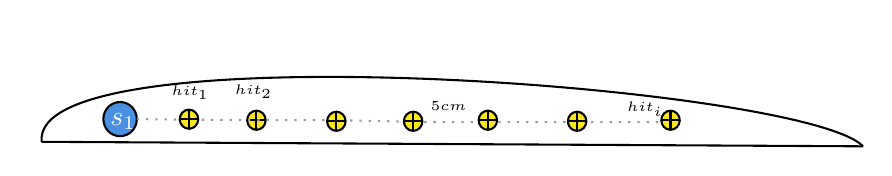
\begin{tikzpicture}[x=0.75pt,y=0.75pt,yscale=-1,xscale=1]
%uncomment if require: \path (0,300); %set diagram left start at 0, and has height of 300

%Curve Lines [id:da8422582381977624] 
\draw    (38.5,121) .. controls (32.24,66.51) and (406.04,93.84) .. (434.24,123.17) ;
%Straight Lines [id:da8049776185709991] 
\draw    (38.5,121) -- (434.24,123.17) ;
%Shape: Ellipse [id:dp7062717290883331] 
\draw  [color={rgb, 255:red, 0; green, 0; blue, 0 }  ,draw opacity=1 ][fill={rgb, 255:red, 74; green, 144; blue, 226 }  ,fill opacity=1 ] (68.2,110.06) .. controls (68.2,105.51) and (71.81,101.83) .. (76.26,101.83) .. controls (80.71,101.83) and (84.32,105.51) .. (84.32,110.06) .. controls (84.32,114.6) and (80.71,118.28) .. (76.26,118.28) .. controls (71.81,118.28) and (68.2,114.6) .. (68.2,110.06) -- cycle ;
\draw  [fill={rgb, 255:red, 248; green, 231; blue, 28 }  ,fill opacity=1 ] (137.5,110.61) .. controls (137.5,108.06) and (139.5,106) .. (141.96,106) .. controls (144.42,106) and (146.41,108.06) .. (146.41,110.61) .. controls (146.41,113.15) and (144.42,115.22) .. (141.96,115.22) .. controls (139.5,115.22) and (137.5,113.15) .. (137.5,110.61) -- cycle ; \draw   (137.5,110.61) -- (146.41,110.61) ; \draw   (141.96,106) -- (141.96,115.22) ;
%Straight Lines [id:da6986266442320166] 
\draw [color={rgb, 255:red, 155; green, 155; blue, 155 }  ,draw opacity=1 ] [dash pattern={on 0.84pt off 2.51pt}]  (84.32,110.06) -- (133.33,110.54) -- (178.33,110.54) -- (223.35,111.48) -- (278.83,111.54) -- (330.85,111.48) -- (337.85,111.48) ;
\draw  [fill={rgb, 255:red, 248; green, 231; blue, 28 }  ,fill opacity=1 ] (105,110.11) .. controls (105,107.56) and (107,105.5) .. (109.46,105.5) .. controls (111.92,105.5) and (113.91,107.56) .. (113.91,110.11) .. controls (113.91,112.65) and (111.92,114.72) .. (109.46,114.72) .. controls (107,114.72) and (105,112.65) .. (105,110.11) -- cycle ; \draw   (105,110.11) -- (113.91,110.11) ; \draw   (109.46,105.5) -- (109.46,114.72) ;
\draw  [fill={rgb, 255:red, 248; green, 231; blue, 28 }  ,fill opacity=1 ] (213,111.11) .. controls (213,108.56) and (215,106.5) .. (217.46,106.5) .. controls (219.92,106.5) and (221.91,108.56) .. (221.91,111.11) .. controls (221.91,113.65) and (219.92,115.72) .. (217.46,115.72) .. controls (215,115.72) and (213,113.65) .. (213,111.11) -- cycle ; \draw   (213,111.11) -- (221.91,111.11) ; \draw   (217.46,106.5) -- (217.46,115.72) ;
\draw  [fill={rgb, 255:red, 248; green, 231; blue, 28 }  ,fill opacity=1 ] (292,111.11) .. controls (292,108.56) and (294,106.5) .. (296.46,106.5) .. controls (298.92,106.5) and (300.91,108.56) .. (300.91,111.11) .. controls (300.91,113.65) and (298.92,115.72) .. (296.46,115.72) .. controls (294,115.72) and (292,113.65) .. (292,111.11) -- cycle ; \draw   (292,111.11) -- (300.91,111.11) ; \draw   (296.46,106.5) -- (296.46,115.72) ;
\draw  [fill={rgb, 255:red, 248; green, 231; blue, 28 }  ,fill opacity=1 ] (337,110.61) .. controls (337,108.06) and (339,106) .. (341.46,106) .. controls (343.92,106) and (345.91,108.06) .. (345.91,110.61) .. controls (345.91,113.15) and (343.92,115.22) .. (341.46,115.22) .. controls (339,115.22) and (337,113.15) .. (337,110.61) -- cycle ; \draw   (337,110.61) -- (345.91,110.61) ; \draw   (341.46,106) -- (341.46,115.22) ;
\draw  [fill={rgb, 255:red, 248; green, 231; blue, 28 }  ,fill opacity=1 ] (249,110.61) .. controls (249,108.06) and (251,106) .. (253.46,106) .. controls (255.92,106) and (257.91,108.06) .. (257.91,110.61) .. controls (257.91,113.15) and (255.92,115.22) .. (253.46,115.22) .. controls (251,115.22) and (249,113.15) .. (249,110.61) -- cycle ; \draw   (249,110.61) -- (257.91,110.61) ; \draw   (253.46,106) -- (253.46,115.22) ;
\draw  [fill={rgb, 255:red, 248; green, 231; blue, 28 }  ,fill opacity=1 ] (176,111.11) .. controls (176,108.56) and (178,106.5) .. (180.46,106.5) .. controls (182.92,106.5) and (184.91,108.56) .. (184.91,111.11) .. controls (184.91,113.65) and (182.92,115.72) .. (180.46,115.72) .. controls (178,115.72) and (176,113.65) .. (176,111.11) -- cycle ; \draw   (176,111.11) -- (184.91,111.11) ; \draw   (180.46,106.5) -- (180.46,115.72) ;

% Text Node
\draw (70.06,105.94) node [anchor=north west][inner sep=0.75pt]  [color={rgb, 255:red, 255; green, 255; blue, 255 }  ,opacity=1 ] [align=left] {$\displaystyle s_{1}$};
% Text Node
\draw (224.5,100) node [anchor=north west][inner sep=0.75pt]  [font=\tiny] [align=left] {$\displaystyle 5cm\ $};
% Text Node
\draw (99.56,92.44) node [anchor=north west][inner sep=0.75pt]  [font=\tiny,color={rgb, 255:red, 0; green, 0; blue, 0 }  ,opacity=1 ] [align=left] {$\displaystyle hit_{1}$};
% Text Node
\draw (130.06,91.94) node [anchor=north west][inner sep=0.75pt]  [font=\tiny,color={rgb, 255:red, 0; green, 0; blue, 0 }  ,opacity=1 ] [align=left] {$\displaystyle hit_{2}$};
% Text Node
\draw (319.06,100.44) node [anchor=north west][inner sep=0.75pt]  [font=\tiny,color={rgb, 255:red, 0; green, 0; blue, 0 }  ,opacity=1 ] [align=left] {$\displaystyle hit_{i}$};


\end{tikzpicture}